\chapter{Introduction}\label{chapt:intro}

Monitoring roads is an essential element in urban planning. Almost every city is developed around centers with adequate transportation facilities. They provide infrastructural support to both the agricultural and industrial sectors of every country. Given its uses in disaster management, transportation of facilities, social interaction, it is historically proven that everything can efficiently work out if we have a proper mapped site. Mapping the roads, thus, is of utmost importance.

Historically, roads were mapped manually using approximate measures, mostly for short distances, and to help religious pilgrims navigate. With the development of automobiles, maps soon became more extensive and kept in the form of books~\cite{firstMapBooks}. These were handwritten until digital maps could be produced. With the help of Global Positing Systems~(GPS) navigation, maps started becoming digital and electronic versions were kept. These electronic versions had many advantages over their paper counterparts. With digital versions, the limitations of paper: wearability, tendency to be lost or damaged easily, is no longer a pressing issue. 

Though the digital versions could now be replicated easily by printers or by transferring files to other supported devices, taking GPS enabled devices to mark roads is both inefficient and costly. Some roads are inaccessible due to various factors. To combat the individual mapping of roads, some open crowdsourcing platforms like \href{https://www.openstreetmap.org/}{OpenStreetMap~(OSM)} help people continue researching by using their data. This successfully reduced the redundant work, but there is no way to check if the data is correct. Almost always, human errors reduce the quality of data. Millions of kilometers of roads are still left to be digitized to be used for any activity~\cite{MapsDoneOSM}. As previous road data might have changed, completing the mapping of the remaining roads still does not guarantee us the latest report.

The computer is one piece of technology which makes our work a lot simpler. With the advent of techniques such as Machine Learning, identifying patterns to solve certain kinds of problems has become a lot easier. This work is an attempt to use image segmentation based on computer vision techniques to detect roads in satellite images. This will help us in reducing the manual workforce to a large extent. While road detection has been extensively documented in research papers, these papers mostly focus on identifying roads while the camera is on the road. While this has it's own uses in navigation, but using these techniques for surveying is not feasible as one will have to drive all the way, resulting in highly inefficient surveying. Some papers have tried to overcome this problem by high-resolution satellite images, but high-resolution images are quite expensive and have to be bought commercially. Another widespread problem these satellite images face is radiometric distortion. Roads of asphalt, sometimes turn from dark grey into bright white due to some reflection affecting satellite sensors. This is seen clearly is \cref{fig:sat_img_radiometric_distortion}~\cite{GF2-imageCaseStudy}. 

\begin{figure}[h!]
  \centering
  \begin{subfigure}{0.48\textwidth}
    \includegraphics[width=\textwidth]{sat_img_GF2_radiometric_distortion}
    \caption{}
  \end{subfigure}~
  \begin{subfigure}{0.48\textwidth}
    \includegraphics[width=\textwidth]{sat_img_zoomed_GF2_radiometric_distrotion}
    \caption{}
  \end{subfigure}
  \caption[Optical distortion clearly visible on roads]{Optical distortion clearly visible on roads. \textbf{(a)}~Radiometric distortion in image from GF2 satellite. \textbf{(b)}~Zoomed image of (a). Taken from~\cite{GF2-imageCaseStudy}.}
  \label{fig:sat_img_radiometric_distortion}
\end{figure}

We will be using mid-resolution satellite images as they can be used for large scale surveys to tackle distortion and reduce the cost. The identification of roads on mid-resolution~(>~5~m) satellite data is difficult and often has low accuracy. A typical two-lane road has a width of around 7~m, and this road will have a width of hardly a pixel in our satellite image. This work is an effort to use image segmentation techniques in the area of remote sensing to detect roads in mid-resolution satellite images.

When applying existing road-detection algorithms to mid-resolution satellite images, the algorithm is able to predict the location of wide roads successfully. What remains an issue are the roads which occupy about 1~pixel in the image. Two reasons can be thought upon for this issue. One hypothesis is that our algorithm is unable to classify the pixel-level road properly. However, it correctly classified the roads which have, say 4~pixels. A filter, if taken appropriate steps, cannot be biased again these roads. Hence, the only possible option is that our filters are unable to detect any edge in the roads occupying just a pixel. The most intuitive way to counter this problem is to break down an individual pixel into $x$ different pixels. This is the same problem that super-resolution promises to solve. Hence, in this work, we try to detect roads using a model consisting of super-resolution and road-detection as its subcomponents.


RGB images from satellite \href{https://sentinel.esa.int/web/sentinel/missions/sentinel-2}{Sentinel-2A} is used in this work-report. \Cref{tab:sentinel-resolution} lists the detailed parameters of the satellite. Band 2 (Blue), 3 (Green), and 4 (Red) are stacked together to get a 3-channel RGB image. As seen in the specifications, the spacial resolution of the final image is 10~m. The task is to increase the accuracy of the existing road-detection algorithm.

\begin{table}[h!]
  \centering
  \begin{tabular}{ |c|c|c| }
    \hline
    Spatial resolution~(m) & Band number & Central wavelength~(nm) \\
    \hline
    10&2&492.4 \\
    10&3&559.8 \\
    10&4&664.6 \\
    10&8&832.8 \\
    20&5&704.1 \\
    20&6&740.5 \\
    20&7&782.8 \\
    20&8a&864.7 \\
    20&11&1613.7 \\
    20&12&2202.4 \\
    60&1&442.7 \\
    60&9&945.1 \\
    60&10&1373.5 \\
    \hline
  \end{tabular}
  \caption[Wavelengths and bandwidths of the three spatial resolutions of the MSI instruments]{Wavelengths and bandwidths of the three spatial resolutions of the MSI instruments~\cite{sentinelSpecifications}.}
  \label{tab:sentinel-resolution}
\end{table}

By combining the three bands from the raw satellite image, the resulting image size is of the order of 400~MB for one mid-sized city. At first, this may not seem significant in comparison with some of the media files. Yet, handling files of this size in DCNN is a severe issue. Processing large files might be possible for massive supercomputers; however a general workstation has Random Access Memory~(RAM) anywhere from 128 to 256~GBs of RAM, while personal computers range from 8~GB to 32~GBs of RAM. Thus, this image must be divided into several parts so that our algorithms work on a readily available device.

Our input image does not have a sufficiently high resolution to identify small roads. To deal with this problem of pixelization, we will be using two types of models. This setup is shown in \cref{fig:model_complete_without_labels}. Unless specifically mentioned, a model means a combined setup using super-resolution and road-detection models. Data from the input layer goes to the super-resolution model, which is consequently passed to the road-detection model. The final output consists of the predicted road network in the image.

\begin{figure}[h!]
  \centering
  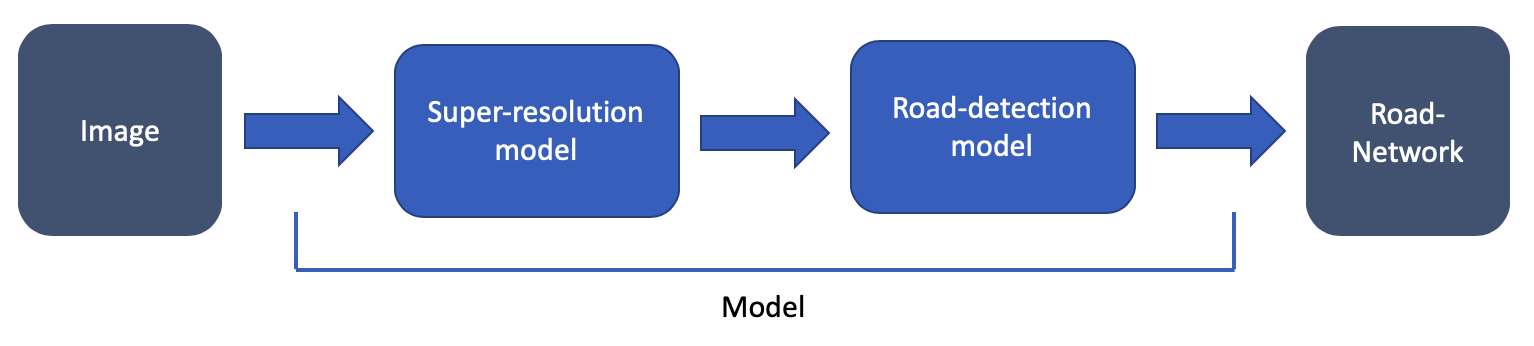
\includegraphics[width=\textwidth]{model_complete_without_labels}
  \caption{Complete setup: Combination of super-resolution and road-detection models.}
  \label{fig:model_complete_without_labels}
\end{figure}
